%
% Packages
%
\documentclass[10pt]{article} 
\usepackage[landscape]{geometry}
\usepackage{url}
\usepackage{multicol}
\usepackage{amsmath}
\usepackage{esint}
\usepackage{bigints}
\usepackage{amsfonts}
\usepackage{xcolor}
\usepackage{tikz}
\usetikzlibrary{calc}
\usetikzlibrary{decorations.pathmorphing}
\usepackage{amsmath,amssymb}
\usepackage{colortbl}
\usepackage{xcolor}
\usepackage{mathtools}
\usepackage{amsmath,amssymb}
\usepackage{enumitem}
\usepackage{xhfill}
\usepackage[french]{babel}
\usepackage[utf8]{inputenc}
\usepackage{parskip}
\usepackage[T1]{fontenc}
\usepackage{mathrsfs}
\usepackage{pgfplots}
\usetikzlibrary{pgfplots.groupplots}
\pgfplotsset{compat=1.17}
\makeatletter


%
% Setup
%
\title{AdMoApp - Olivier D'Ancona}
\advance\topmargin-.8in
\advance\textheight3in
\advance\textwidth3in
\advance\oddsidemargin-1.5in
\advance\evensidemargin-1.5in
\setlength{\parindent}{0pt} % No indentation at the start of a paragraph
\setlength{\parskip}{6pt plus 2pt minus 1pt} % Space between paragraphs

\baselineskip2pt
\linespread{0.4}
\setlength{\abovedisplayskip}{3pt}
\setlength{\belowdisplayskip}{3pt}
\setlength{\abovedisplayshortskip}{3pt}
\setlength{\belowdisplayshortskip}{3pt}


%
% Commands
%
\newcommand*\bigcdot{\mathpalette\bigcdot@{.5}}
\newcommand*\bigcdot@[2]{\mathbin{\vcenter{\hbox{\scalebox{#2}{$\m@th#1\bullet$}}}}}
\makeatother
\newcommand{\hr}{\centerline{\rule{3.5in}{1pt}}}
%\colorbox[HTML]{e4e4e4}{\makebox[\textwidth-2\fboxsep][l]{texto}
\newcommand{\nc}[2][]{%
\vspace{-.16cm}
\tikz \draw [draw=black, ultra thick, #1]
    ($(current page.center)-(0.5\linewidth,0)$) --
    ($(current page.center)+(0.5\linewidth,0)$)
    node [midway, fill=white] {#2};
}% tomado de https://tex.stackexchange.com/questions/179425/a-new-command-of-the-form-tex


%
% Styles
%
\tikzstyle{mybox} = [draw=black, fill=white, very thick,
rectangle, rounded corners, inner sep=2pt, inner ysep=7pt]
\tikzstyle{fancytitle} =[fill=black, text=white, font=\bfseries]

\newlength{\boxsize}
\setlength{\boxsize}{0.247\textwidth}
\raggedcolumns
%###############################################################################################
%
%                                         Document
%
%###############################################################################################



\begin{document}

%---------------------------------
% Title
%---------------------------------
\begin{center}
    {\huge{\textbf{AdMoApp - Olivier D'Ancona}}}\\
\end{center}
\vspace{-0.1cm}

\begin{multicols*}{4}
    
    %---------------------------------
    % Clean Architecture
    %---------------------------------
    \begin{tikzpicture}
        \node [mybox] (box){%
            \begin{minipage}{0.247\textwidth}
                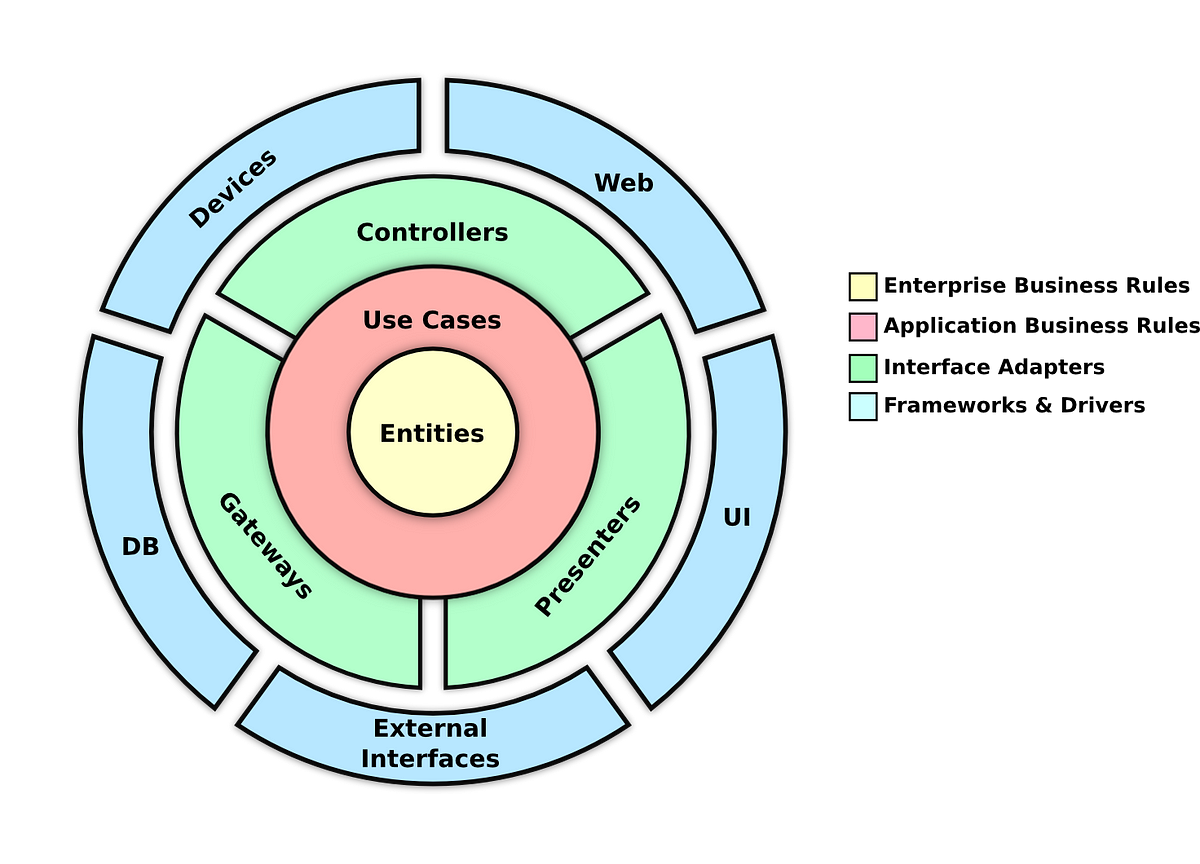
\includegraphics[width=\textwidth]{images/clean_architecture.png}
                \textbf{Data Layer} : Includes Repositories and Data Sources. Repositories contain
                queries and change of specific data model. Can decide
                which data source to choose (network or BD)\\
                \textbf{Domain Layer} : Contains Model and Uses Cases. Use cases combine data
                from repositories and extract the business logic from the view
                models.\\
                \textbf{Presentation Layer} : UI, ViewModels, etc.\\
                \nc{implementation}
                Data Flow: depends on data Layer
                Depedency Rule: depends on domain
            \end{minipage}
        };
        \node[fancytitle, right=10pt] at (box.north west) {Clean Architecture};
    \end{tikzpicture}
    %---------------------------------
    
    %---------------------------------
    % MMVM
    %---------------------------------
    \begin{tikzpicture}
        \node [mybox] (box){%
            \begin{minipage}{0.247\textwidth}
                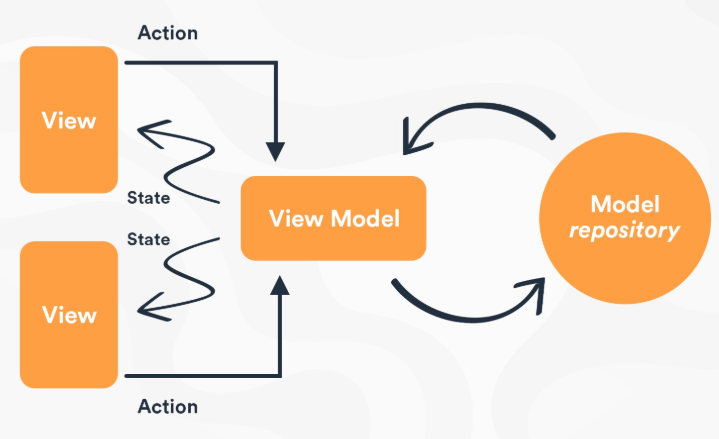
\includegraphics[width=\textwidth]{images/mvvm.png}
            \end{minipage}
        };
        \node[fancytitle, right=10pt] at (box.north west) {MMVM};
    \end{tikzpicture}
    %---------------------------------
    
    %---------------------------------
    % Widget
    %---------------------------------
    \begin{tikzpicture}
        \node [mybox] (box){%
            \begin{minipage}{0.247\textwidth}
                \nc{Stateless}
                Widget that does not require a mutable state. Useful to describe static UI.\\
                \nc{Stateful}
                Widget that has a mutable state. Useful to describe dynamic UI.\\
                \nc{Inherited}
            \end{minipage}
        };
        \node[fancytitle, right=10pt] at (box.north west) {Widget};
    \end{tikzpicture}
    %---------------------------------
    
    %---------------------------------
    % Null Safety
    %---------------------------------
    \begin{tikzpicture}
        \node [mybox] (box){%
            \begin{minipage}{0.247\textwidth}
                When you opt into null safety, types in your code are non-nullable by
                default, meaning that variables can't contain null unless you say they
                can. With null safety, your runtime null-dereference errors turn into edittime analysis errors.
                ? => nullable
                ! => non-nullable
            \end{minipage}
        };
        \node[fancytitle, right=10pt] at (box.north west) {Null Safety};
    \end{tikzpicture}
    %---------------------------------
    
    %---------------------------------
    % Provider
    %---------------------------------
    \begin{tikzpicture}
        \node [mybox] (box){%
            \begin{minipage}{0.247\textwidth}
            \end{minipage}
        };
        \node[fancytitle, right=10pt] at (box.north west) {Provider};
    \end{tikzpicture}
    %---------------------------------
    
    %---------------------------------
    % Stream
    %---------------------------------
    \begin{tikzpicture}
        \node [mybox] (box){%
            \begin{minipage}{0.247\textwidth}
            \end{minipage}
        };
        \node[fancytitle, right=10pt] at (box.north west) {Stream};
    \end{tikzpicture}
    %---------------------------------
    
    %---------------------------------
    % Future
    %---------------------------------
    \begin{tikzpicture}
        \node [mybox] (box){%
            \begin{minipage}{0.247\textwidth}
            \end{minipage}
        };
        \node[fancytitle, right=10pt] at (box.north west) {Future};
    \end{tikzpicture}
    %---------------------------------
    
    %---------------------------------
    % Api
    %---------------------------------
    \begin{tikzpicture}
        \node [mybox] (box){%
            \begin{minipage}{0.247\textwidth}
            \end{minipage}
        };
        \node[fancytitle, right=10pt] at (box.north west) {Api};
    \end{tikzpicture}
    %---------------------------------
    
    %---------------------------------
    % Storage
    %---------------------------------
    \begin{tikzpicture}
        \node [mybox] (box){%
            \begin{minipage}{0.247\textwidth}
            \end{minipage}
        };
        \node[fancytitle, right=10pt] at (box.north west) {Storage};
    \end{tikzpicture}
    %---------------------------------
    
    %---------------------------------
    % Json
    %---------------------------------
    \begin{tikzpicture}
        \node [mybox] (box){%
            \begin{minipage}{0.247\textwidth}
            \end{minipage}
        };
        \node[fancytitle, right=10pt] at (box.north west) {Json};
    \end{tikzpicture}
    %---------------------------------
    
    %---------------------------------
    % Cubit
    %---------------------------------
    \begin{tikzpicture}
        \node [mybox] (box){%
            \begin{minipage}{0.247\textwidth}
            \end{minipage}
        };
        \node[fancytitle, right=10pt] at (box.north west) {Cubit};
    \end{tikzpicture}
    %---------------------------------
    
    %---------------------------------
    % Bloc
    %---------------------------------
    \begin{tikzpicture}
        \node [mybox] (box){%
            \begin{minipage}{0.247\textwidth}
            \end{minipage}
        };
        \node[fancytitle, right=10pt] at (box.north west) {Bloc};
    \end{tikzpicture}
    %---------------------------------
    
    %---------------------------------
    % Action Theory
    %---------------------------------
    \begin{tikzpicture}
        \node [mybox] (box){%
            \begin{minipage}{0.247\textwidth}
            \end{minipage}
        };
        \node[fancytitle, right=10pt] at (box.north west) {Action Theory};
    \end{tikzpicture}
    %---------------------------------
    
    %---------------------------------
    % Golden Rules
    %---------------------------------
    \begin{tikzpicture}
        \node [mybox] (box){%
            \begin{minipage}{0.247\textwidth}
            \end{minipage}
        };
        \node[fancytitle, right=10pt] at (box.north west) {Golden Rules};
    \end{tikzpicture}
    %---------------------------------
    
    %---------------------------------
    % Norman Principles
    %---------------------------------
    \begin{tikzpicture}
        \node [mybox] (box){%
            \begin{minipage}{0.247\textwidth}
            \end{minipage}
        };
        \node[fancytitle, right=10pt] at (box.north west) {Norman Principles};
    \end{tikzpicture}
    %---------------------------------
    
    %---------------------------------
    % Action Theory
    %---------------------------------
    \begin{tikzpicture}
        \node [mybox] (box){%
            \begin{minipage}{0.247\textwidth}
            \end{minipage}
        };
        \node[fancytitle, right=10pt] at (box.north west) {Action Theory};
    \end{tikzpicture}
    %---------------------------------
    
    %---------------------------------
    % Loi de Fitts
    %---------------------------------
    \begin{tikzpicture}
        \node [mybox] (box){%
            \begin{minipage}{0.247\textwidth}
                $$MT = a + b \cdot \log2\left(\frac{2D}{w}\right)$$
            \end{minipage}
        };
        \node[fancytitle, right=10pt] at (box.north west) {Loi de Fitts};
    \end{tikzpicture}
    %---------------------------------
    
    %---------------------------------
    % Usability
    %---------------------------------
    \begin{tikzpicture}
        \node [mybox] (box){%
            \begin{minipage}{0.247\textwidth}
            \end{minipage}
        };
        \node[fancytitle, right=10pt] at (box.north west) {Usability (Nielson)};
    \end{tikzpicture}
    %---------------------------------
    
    %---------------------------------
    % Wearables
    %---------------------------------
    \begin{tikzpicture}
        \node [mybox] (box){%
            \begin{minipage}{0.247\textwidth}
            \end{minipage}
        };
        \node[fancytitle, right=10pt] at (box.north west) {Wearables};
    \end{tikzpicture}
    %---------------------------------
    
    %---------------------------------
    % Ergonomic Criteria (Bastien Scapin)
    %---------------------------------
    \begin{tikzpicture}
        \node [mybox] (box){%
            \begin{minipage}{0.247\textwidth}
            \end{minipage}
        };
        \node[fancytitle, right=10pt] at (box.north west) {Ergonomic Criteria (Bastien Scapin)};
    \end{tikzpicture}
    %---------------------------------
    
    %---------------------------------
    % Context
    %---------------------------------
    \begin{tikzpicture}
        \node [mybox] (box){%
            \begin{minipage}{0.247\textwidth}
                
            \end{minipage}
        };
        \node[fancytitle, right=10pt] at (box.north west) {Context};
    \end{tikzpicture}
    %---------------------------------
    
    %---------------------------------
    % System Usability Scale
    %---------------------------------
    \begin{tikzpicture}
        \node [mybox] (box){%
            \begin{minipage}{0.247\textwidth}
                \begin{enumerate}[noitemsep]
                    \item Like to use frequently
                    \item Too complex
                    \item Easy to use
                    \item Need Assistance
                    \item Functions well integrated
                    \item Consistent
                    \item Learn quickly
                    \item Efficient
                    \item Easy to remember
                    \item Could be more enjoyable
                \end{enumerate}
            \end{minipage}
        };
        \node[fancytitle, right=10pt] at (box.north west) {System Usability Scale};
    \end{tikzpicture}
    %---------------------------------
    
    
    %---------------------------------
    % Cognitive WalkThrough
    %---------------------------------
    \begin{tikzpicture}
        \node [mybox] (box){%
            \begin{minipage}{0.247\textwidth}
                At each step, ask the following questions:
                \begin{enumerate}[noitemsep]
                    \item Will the user try to achieve the correct effect?
                    \item Will the user notice that the correct action is available?
                    \item Will the user associate the correct action with the effect that user is trying to achieve?
                    \item If the correct action is performed, will the user see that progress is being made toward solution of the task?
                \end{enumerate}
            \end{minipage}
        };
        \node[fancytitle, right=10pt] at (box.north west) {Cognitive WalkThrough};
    \end{tikzpicture}
    %---------------------------------
    
    %---------------------------------
    % Heuristics
    %---------------------------------
    \begin{tikzpicture}
        \node [mybox] (box){%
            \begin{minipage}{0.247\textwidth}
                \begin{enumerate}[noitemsep]
                    \item Status Visibility
                    \item Match between system and real world
                    \item User control and freedom
                    \item Consistency and standards
                    \item Error prevention
                    \item Recognition rather than recall
                    \item Flexibility and efficiency of use
                    \item Aesthetic and minimalist design
                    \item Help users recognize, diagnose, and recover from errors
                    \item Help and documentation
                \end{enumerate}
            \end{minipage}
        };
        \node[fancytitle, right=10pt] at (box.north west) {Heuristics};
    \end{tikzpicture}
    %---------------------------------
    
    
    
\end{multicols*}

\end{document}